% Physics of Complex Networks -- Theoretical project
% Synchronisation as diffusion geometry
\documentclass[twocolumn,aps,prl,superscriptaddress,nofootinbib]{revtex4-2}

\usepackage{graphicx}
\usepackage{amsmath,amssymb}
\usepackage{bm}
\usepackage{booktabs}
\usepackage{amsthm}
\usepackage[colorlinks=true,linkcolor=blue,citecolor=blue]{hyperref}

\graphicspath{{figures/}{../../images/}{../figures/}}

% --- theorem environments -----------
\theoremstyle{plain}
\newtheorem{lemma}{Lemma}
\newtheorem{corollary}[lemma]{Corollary}
\newtheorem{proposition}[lemma]{Proposition}
\theoremstyle{definition}
\newtheorem{definition}{Definition}

\newcommand{\Lap}{\mathsf{L}}
\newcommand{\Adj}{\mathsf{A}}
\newcommand{\Deg}{\mathsf{D}}
\newcommand{\Cov}{\mathsf{C}}
\newcommand{\deff}{d_{\mathrm{eff}}}
\newcommand{\Lrw}{\Lap_{\mathrm{rw}}}

% \nofiles
\begin{document}

\title{Synchronisation as Diffusion Geometry: Topological Scales in Modular Networks}
\author{Filippo Bezzi}
\affiliation{Physics of Complex Networks, Universit\`a degli Studi di Padova}
\date{\today}

\begin{abstract}
We examine the hypothesis by which transient synchronisation in the Kuramoto model reveals hierarchical community structure in complex networks. In the linearised regime around the steady state, we prove an exact analytical identity demonstrating that the pairwise order parameter $\rho_{ij}(t) = \langle \cos(\theta_i - \theta_j) \rangle$ is equivalent to a diffusion-map kernel $\exp(-d_t^2(i,j)/2)$, where $d_t(i,j)$ is the network's diffusion distance at time $t$. We validate this identity on a synthetic two-level hierarchical network ($N=256$, $z_{\mathrm{in}1}=13, z_{\mathrm{in}2}=4, z_{\mathrm{out}}=1$) using RK4 numerical simulations. By comparing the Laplacian spectrum against a degree-preserving null model and computing the Inverse Participation Ratio (IPR), we separate delocalised structural modes from localized bulk noise. We show that spectral gaps dictate transient plateaus in single-linkage component counts. Furthermore, we analyze two key failure mechanisms of synchronization: targeted degree heterogeneity (hubs), where adding 8 hubs ($\sim 3\%$ of nodes) destroys plateau formation by placing hubs at the diffusion centroid, and structural noise injection (increasing $z_{\mathrm{out}}$), showing that plateau visibility degrades before the spectral gaps collapse.
\end{abstract}

\maketitle

%======================================================================
\paragraph{Introduction}
Understanding the relationship between network topology and dynamic processes is a central theme in network science \cite{arenas2008}. In a landmark paper, Arenas \textit{et al.} \cite{arenas2006} demonstrated that the transient dynamics of Kuramoto oscillators on complex networks reveals community structure, with synchronization dynamics characterized by multiple hierarchical time scales, governed by gaps in the Laplacian spectrum.

In this work, we establish that in the linearised regime, the order parameter proposed by Arenas \textit{et al.} is not merely a definition, but is an exact identity with the diffusion-map kernel introduced by Coifman and Lafon \cite{coifman2006}.

We perform a rigorous evaluation of this framework on a planted 13-4 hierarchical network ($N=256$), validating the analytical identity, characterizing the spectral structure with degree-preserving null models, measuring eigenvector participation ratios \cite{pradhan2017}, tracking single-linkage dendrogram clustering \cite{sibson1973}, evaluating Normalized Mutual Information (NMI) \cite{danon2005}, and investigating failure mechanisms under hub contamination and noise injection sweeps.

%======================================================================
%\section{Task 1: From Kuramoto Transient to Diffusion Distance}
%\label{sec:theory}

\paragraph{Linearised Dynamics of Kuramoto Model}
Consider identical Kuramoto oscillators with natural frequencies $\omega_i = \omega$ on an unweighted, connected graph with adjacency matrix $\Adj$ and degree matrix $\Deg$:
\begin{equation}
\dot{\theta}_i = \omega + K \sum_{j=1}^N A_{ij} \sin(\theta_j - \theta_i).
\label{eq:kuramoto_intro}
\end{equation}
In the co-rotating frame ($\theta_i \mapsto \theta_i - \omega t$) and for small phase differences $\Delta_{ij} = \theta_i - \theta_j$, $\sin(\Delta_{ji}) \approx \theta_j - \theta_i$, yielding the linearised dynamical system:
\begin{equation}
\dot{\bm\theta} = -K\,\Lap\,\bm\theta,
\qquad \Lap=\Deg-\Adj,
\qquad \bm\theta(t)=e^{-K\Lap t}\bm\theta(0).
\label{eq:heat}
\end{equation}
The solution is governed by the Laplacian eigenpairs $\{\lambda_\alpha, \bm v_\alpha\}_{\alpha=1}^N$, ordered such that $0 = \lambda_1 < \lambda_2 \le \dots \le \lambda_N$, assuming only one connected component is present.

Taking Gaussian initial conditions $\bm\theta(0) \sim \mathcal{N}(0, \sigma^2 \mathbb{I})$, the phase vector $\bm\theta(t)$ remains Gaussian with covariance matrix \textsc{$\Cov(t) = \sigma^2 e^{-2K\Lap t}$.} The phase difference $\Delta_{ij} = (\bm e_i - \bm e_j)^\top \bm\theta(t)$ is a zero-mean Gaussian variable with variance $s_{ij}^2 = C_{ii} + C_{jj} - 2C_{ij}$. Evaluating the characteristic function $\langle e^{i \Delta_{ij}} \rangle = \exp(-s_{ij}^2/2)$, we find:
\begin{equation}
\rho_{ij}(t) = \langle \cos(\theta_i - \theta_j) \rangle = \exp\Big( -\frac{1}{2} d_t^2(i,j) \Big),
\label{eq:main_identity}
\end{equation}
where the diffusion distance $d_t(i,j)$ is given by:
\begin{equation}
d_t^2(i,j) = \sigma^2 \sum_{\alpha=2}^N e^{-2K\lambda_\alpha t} \big( \bm v_\alpha(i) - \bm v_\alpha(j) \big)^2,
\label{eq:diff_dist_formula}
\end{equation}
assuming eigenmode $\bm{v}_1(i)=\bm{v}_1(j)$ for all node pairs $(i,j)$ in connected networks (see Appendix~\ref{app:derivation}).
Equation~\eqref{eq:main_identity} establishes that the order parameter $\rho_{ij}(t)$ is exactly the Gaussian diffusion kernel associated with the diffusion map $\Psi_t(i) = \sigma (e^{-K\lambda_2 t} v_2(i), \dots, e^{-K\lambda_N t} v_N(i))$ \cite{coifman2006}.

\paragraph{Spectral Gaps, Plateaus, and Effective Dimension}
From \eqref{eq:heat}, using symmetricity of the Laplacian  we find a decoupled closed form solution for the phase vector $\bm\theta(t)$ as:
\begin{equation}
\theta_i(t)=\sum_{\alpha=1}^N e^{-2K\lambda_{\alpha} t}\bm{v}_{\alpha}(i)\theta_i(0).
\label{eq:closed_form}
\end{equation}
When a spectral gap $\lambda_m \ll \lambda_{m+1}$ exists, modes $\alpha \ge m+1$ decay quickly while modes $\alpha \le m$ remain active over the time window:
\begin{equation}
\frac{1}{2K\lambda_{m+1}} \ll t \ll \frac{1}{2K\lambda_m}.
\end{equation}
Over this window, the diffusion distance matrix $d_t(i,j)$ remains approximately constant across pairs, producing a stable plateau of $m$ clusters. The length of this plateau in logarithmic time $\log_{10} t$ is $\log_{10}(\lambda_{m+1}/\lambda_m)$.

To track the decay of active eigenmodes, we define the spectral mode weights $p_\alpha(t)$ and the effective embedding dimension $\deff(t)$:
\begin{equation}
p_\alpha(t)=\frac{e^{-2K\lambda_\alpha t}}{\sum_{\beta\ge2}e^{-2K\lambda_\beta t}},
\qquad
\deff(t)=\exp\Big[-\sum_{\alpha\ge2}p_\alpha\ln p_\alpha\Big].
\label{eq:deff}
\end{equation}
$\deff(t)$ measures the exponentiated Shannon entropy of active modes, serving as a continuous proxy for the number of communities.

%======================================================================
\paragraph{Validation on Hierarchical Networks}
%\label{sec:validation}

\begin{figure*}[t]
  \centering
  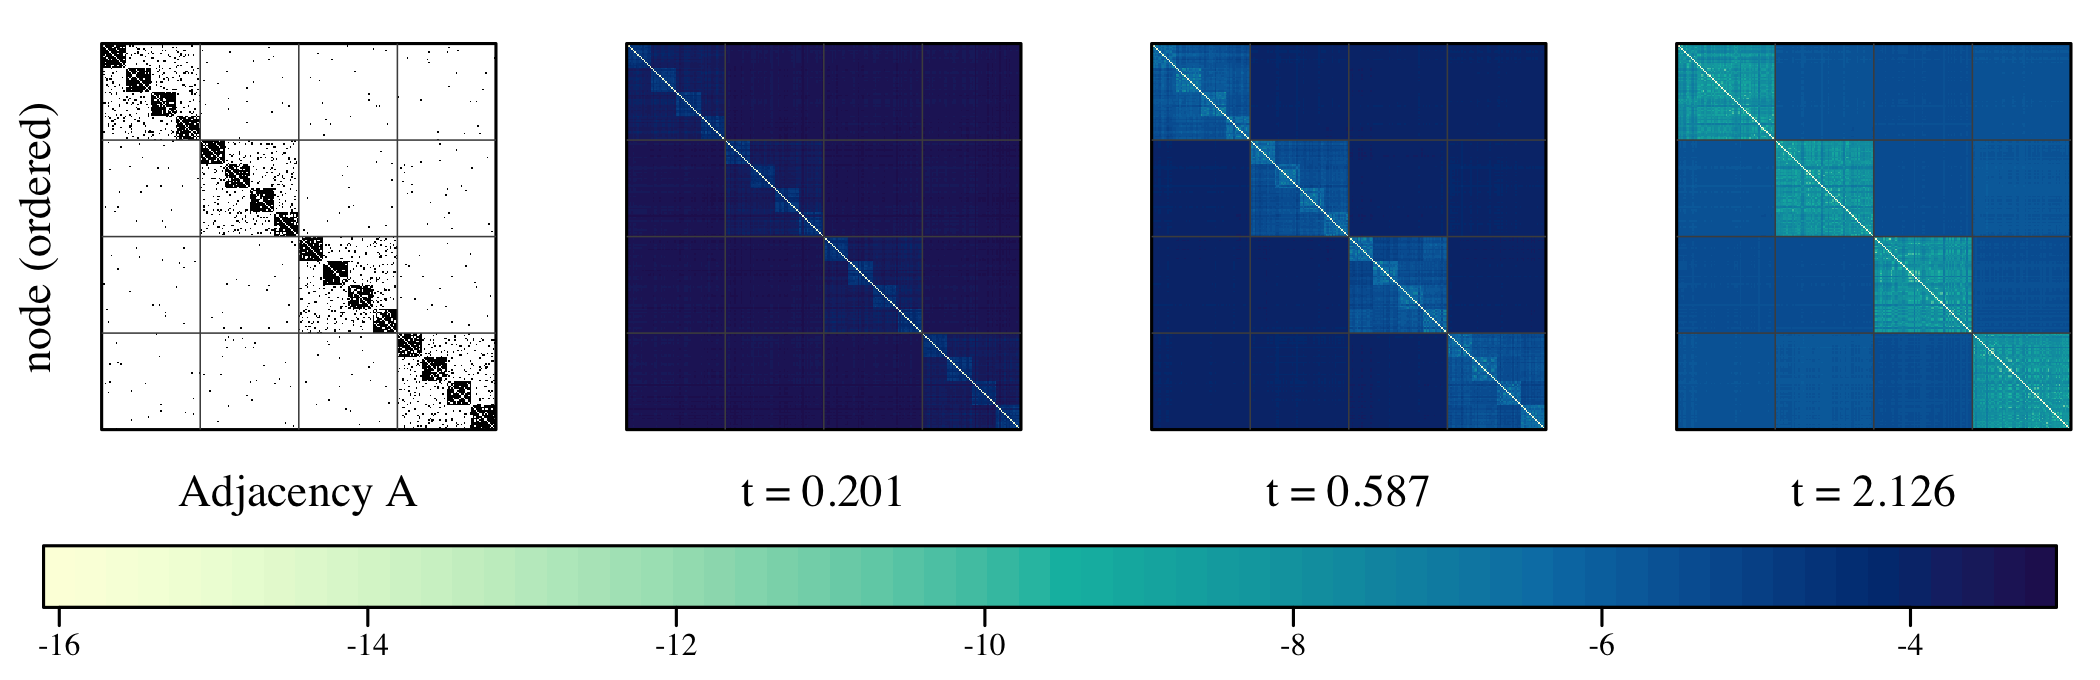
\includegraphics[width=0.98\textwidth]{F1_rho_heatmaps.png}
  \caption[Adjacency and dissimilarity heatmaps]{Adjacency matrix and synchronization dissimilarity heatmaps across time for the 13-4 hierarchical network. From left to right: planted adjacency matrix $\Adj$, and dissimilarity heatmaps $\log_{10}(1-\rho_{ij}(t))$ at times $t = 0.201$, $t = 0.587$, and $t = 2.126$. Light regions indicate high phase synchronisation. Nodes are ordered by planted community structure.}
  \label{fig:rho}
\end{figure*}

We validate the identity $\rho_{ij}(t) = \exp(-d_t^2(i,j)/2)$ on a 2-level hierarchical network ($N=256$) generated by a stochastic block model \cite{arenas2006}. The network consists of 16 first-level communities of 16 nodes, grouped 4-into-1 into 4 second-level communities of 64 nodes. The expected internal and external degrees are $z_{\mathrm{in}1}=13$, $z_{\mathrm{in}2}=4$, and $z_{\mathrm{out}}=1$, giving a theoretical degree expectation $\mathbb{E}[k] = 18$.

We integrate the full non-linear Kuramoto model \eqref{eq:kuramoto_intro} using a vectorized 4th-order Runge-Kutta (RK4) scheme over $M=400$ ensemble members with Gaussian initial phases $\theta_i(0) \sim \mathcal{N}(0, \sigma^2)$ ($\sigma=0.15$) and coupling $K=1.0$.

Figure~\ref{fig:rho} displays the true adjacency matrix $\Adj$ alongside numerical dissimilarity heatmaps $\log_{10}(1-\rho_{ij}(t))$ evaluated across time. The time snapshots ($t=0.201$, $t=0.587$, and $t=2.126$) are extracted from a logarithmic time sampling $t_s \in [0.01, 5.01]$ ($s=1..30$). At early times ($t=0.201$, second panel), phase correlation builds sharply within the 16 micro-communities of size 16. At intermediate times ($t=0.587$, third panel), the micro-communities coalesce into the 4 meso-level blocks of size 64. At later times ($t=2.126$, fourth panel), off-community phase differences decay as the system transitions toward global phase lock. Comparing the empirical average obtained from the full non-linear RK4 Kuramoto simulation $\rho_{ij}^{\mathrm{sim}}(t)$ against the theoretical linear identity $\rho_{ij}^{\mathrm{lin}}(t)$, the pair-wise root-mean-square error $\mathrm{RMS}(t) = \sqrt{\sum_{i,j}(\rho_{ij}^{\mathrm{sim}} - \rho_{ij}^{\mathrm{lin}})^2}/N$ drops below $10^{-4}$ for $t \ge 0.106$ ($\mathrm{RMS} = 7.88 \times 10^{-5}$ at $t=0.106$, and $\mathrm{RMS} = 4.20 \times 10^{-6}$ at $t=0.587$).

%======================================================================
\paragraph{Spectral Gaps and Eigenvector Analysis}
% \label{sec:plateaus}

\begin{figure*}[t]
  \centering
  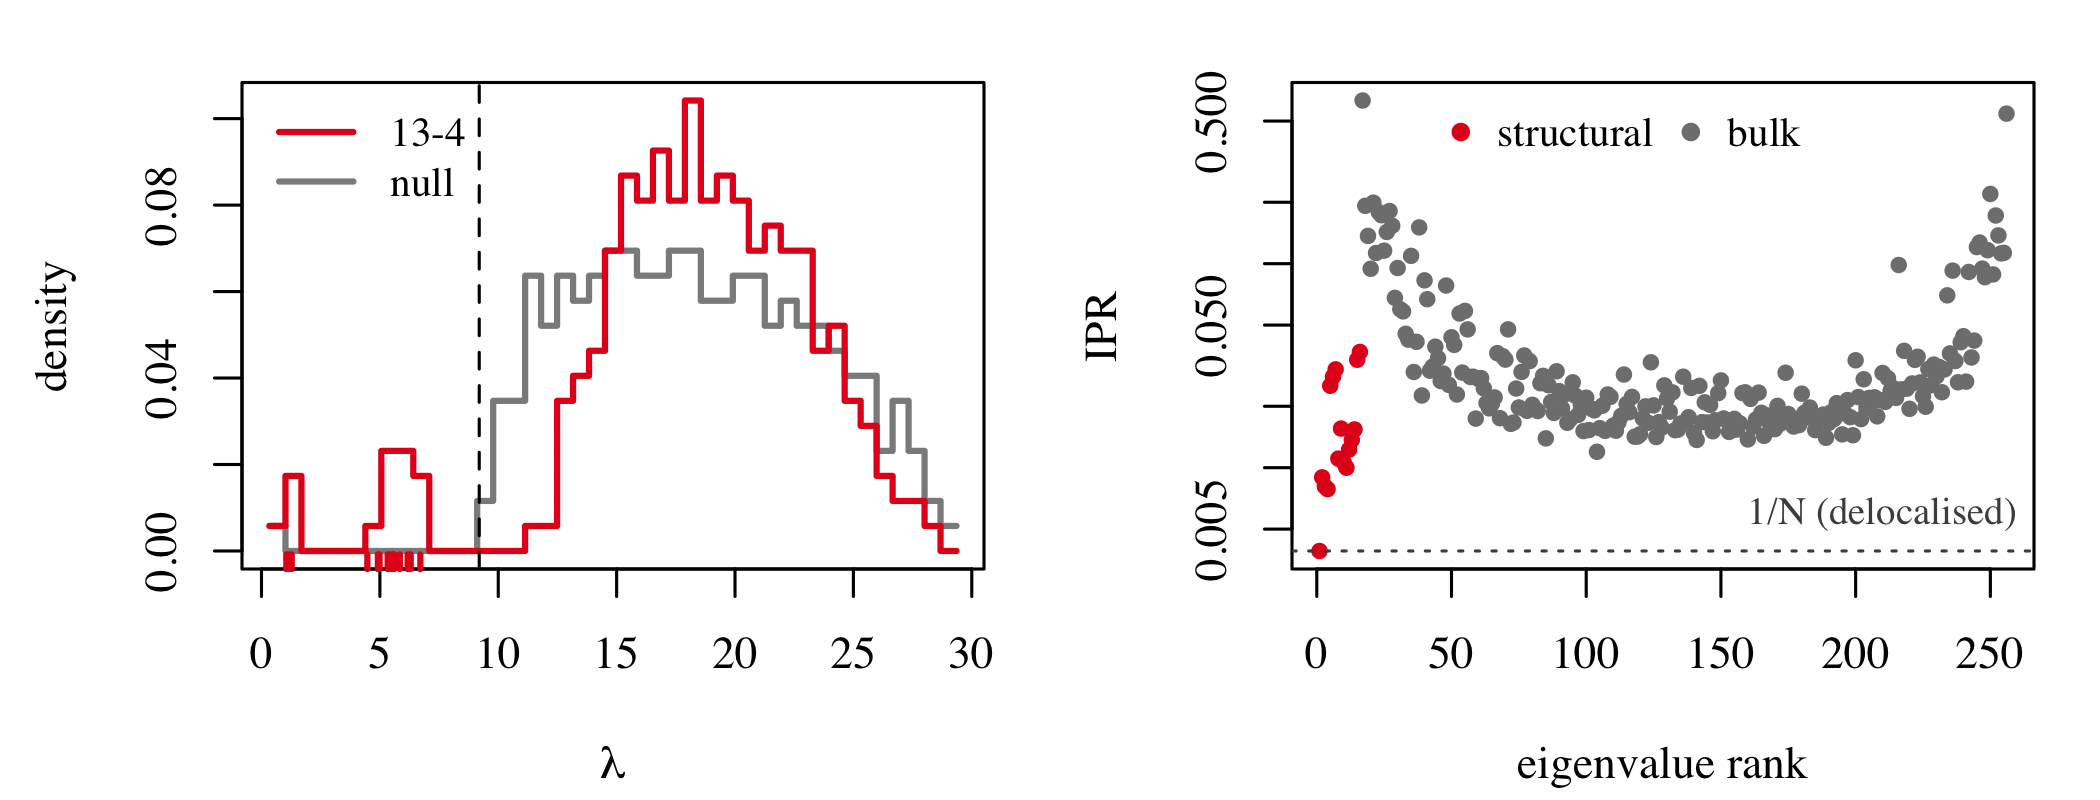
\includegraphics[width=0.98\textwidth]{F2_spectrum.png}
  \caption[Spectral density and IPR]{Spectral properties of the 13-4 hierarchical network versus the degree-preserving null model. Left: Spectral density of the real network (red line) compared against the null model (grey histogram) and the bulk edge $\lambda_{\mathrm{bulk}} = 9.20$ (dashed line). Right: Inverse Participation Ratio (IPR) per mode rank, highlighting that all 16 structural modes ($\lambda < \lambda_{\mathrm{bulk}}$, red points) are delocalised ($\mathrm{IPR} \approx 1/N$), whereas bulk modes (grey points) are localised.}
  \label{fig:spectrum_null}
\end{figure*}

To show the validity of using the spectrum of the linearized Kuramoto model for community detection, we compare the spectrum of the real 13-4 network against a degree-preserving null model generated via double-edge swaps \cite{maslov2002} with $n_{\mathrm{swap}} = 20 E$, where $E$ is the number of edges. This method preserves node degrees while destroying hierarchical structure, allowing us to separate informative structural modes from uninformative random graph fluctuations (``bulk noise").

As shown in Figure~\ref{fig:spectrum_null} (Left), the real spectrum contains 16 eigenvalues lying strictly below the algebraic connectivity of the randomized graph ($\lambda_{\mathrm{bulk}} = 9.20$). To further characterize these modes, we compute the Inverse Participation Ratio (IPR) \cite{pradhan2017}:
\begin{equation}
\mathrm{IPR}(\alpha) = \sum_{i=1}^N v_\alpha(i)^4,
\label{eq:ipr}
\end{equation}
which quantifies the fraction of the graph's nodes on which a given mode is significantly localized. Intuitively, a mode is localized if its amplitude is significant on a small fraction of the graph's nodes, and delocalized if its amplitude is significant on a large fraction of the graph's nodes, with delocalization associated with community structure. In Figure~\ref{fig:spectrum_null} (Right), all 16 structural modes display $\mathrm{IPR} \approx 1/256$, proving that they are delocalised community modes rather than localized hub fluctuations. Furthermore the gap between rank 16 and rank 17 modes confirms that the first 16 modes belong to a completely distinct physical regime.

\begin{figure*}[t]
  \centering
  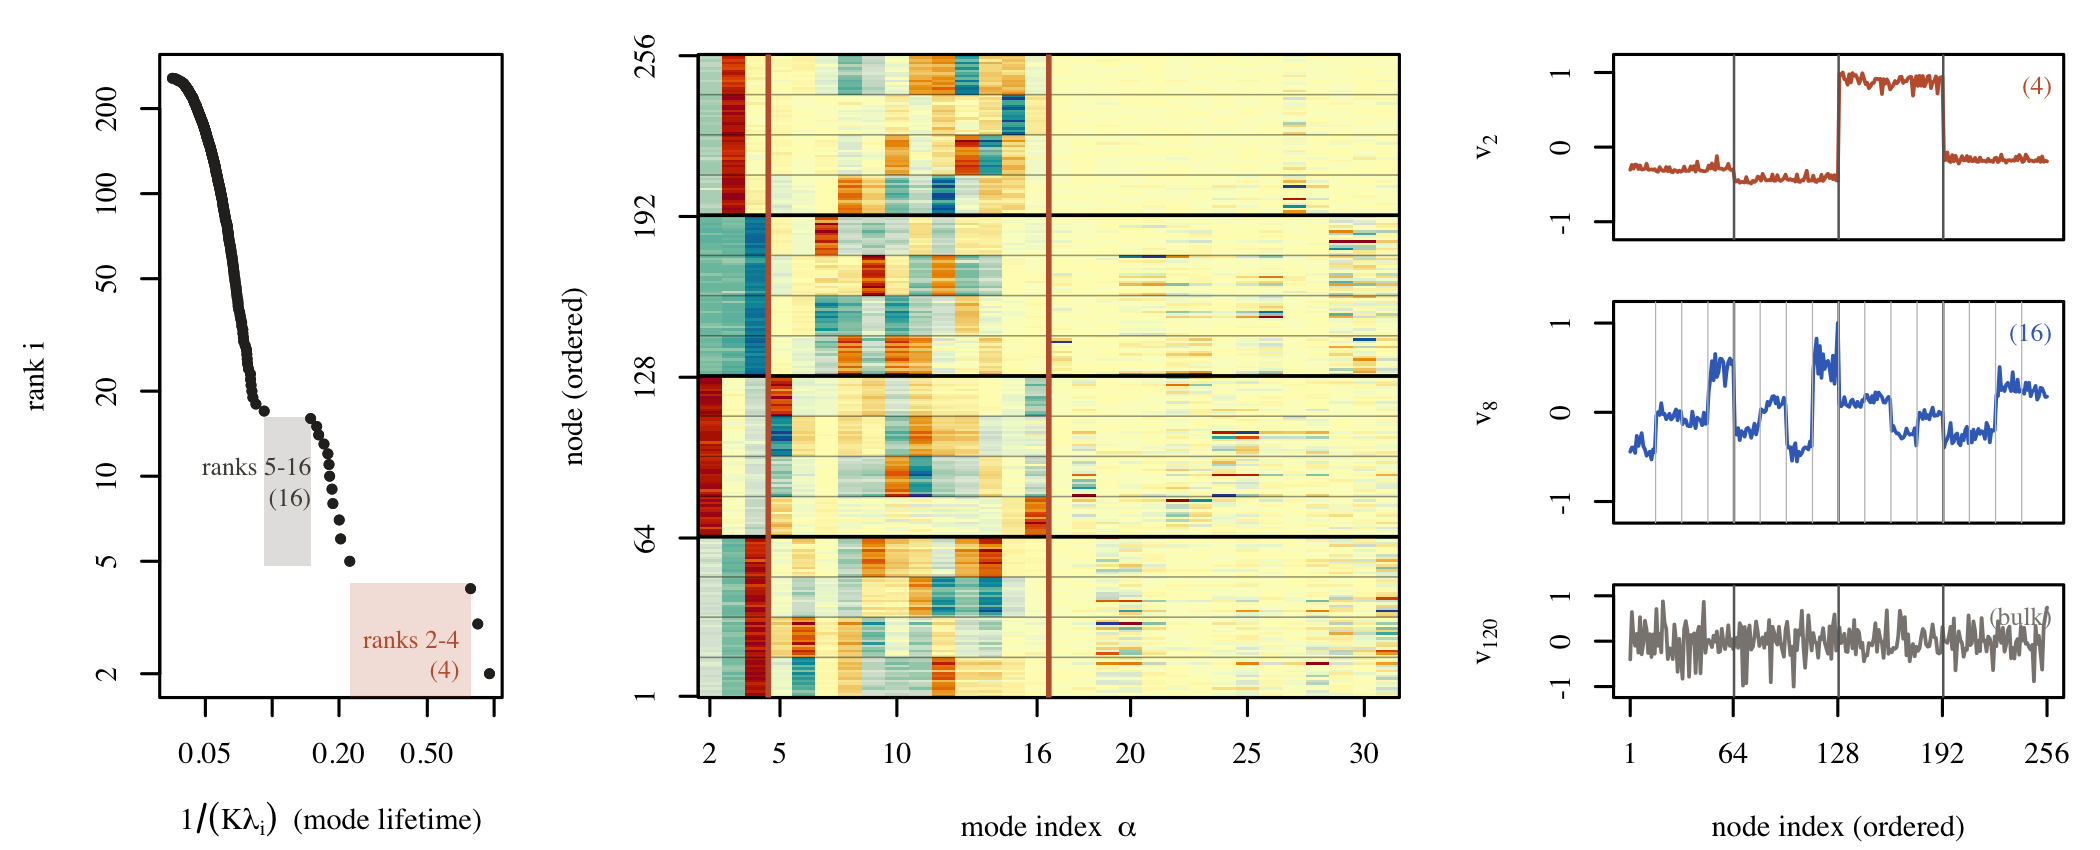
\includegraphics[width=0.98\textwidth]{F3_eigenvectors.png}
  \caption[Eigenvector analysis for 13-4 network]{Eigenvector analysis for the 13-4 hierarchical network. Left: Mode lifetimes $1/(K\lambda_i)$ versus eigenvalue rank $i$, with shaded spectral gap regions for 4 and 16 communities. Center: Eigenvector matrix heatmap $v_\alpha(i)$ across node indices $\alpha=2..31$. Right: Individual eigenvector profiles for $v_2$ (4 blocks), $v_8$ (16 blocks), and $v_{120}$ (bulk mode).}
  \label{fig:eigvec}
\end{figure*}

Figure~\ref{fig:eigvec} provides a detailed view of the eigenvectors. Left panel plots mode lifetimes $1/(K\lambda_i)$, highlighting the leading spectral gaps at $m=4$ ($\lambda_5/\lambda_4 = 3.64$) and $m=16$ ($\lambda_{17}/\lambda_{16} = 1.64$). Center panel displays the eigenvector matrix $v_\alpha(i)$ for modes $\alpha=2..31$. Modes $\alpha=2..4$ are strictly constant on the 4 large blocks, while modes $\alpha=5..16$ are constant on the 16 small blocks. Right panel shows individual mode profiles $v_2(i), v_8(i), v_{120}(i)$, confirming the block-wise low-frequency structure of the structural modes and the high-frequency noise of the bulk mode $v_{120}$. This is also in agreement with the diffusion embeddig distance of \ref{eq:diff_dist_formula}, providing us with a geometrical picture of how the synchronization dynamics on the network are mapped to the diffusion embedding space.

%======================================================================
\paragraph{Component Plateaus and Diffusion Geometry}
%\label{sec:embedding}

\begin{figure*}[t]
  \centering
  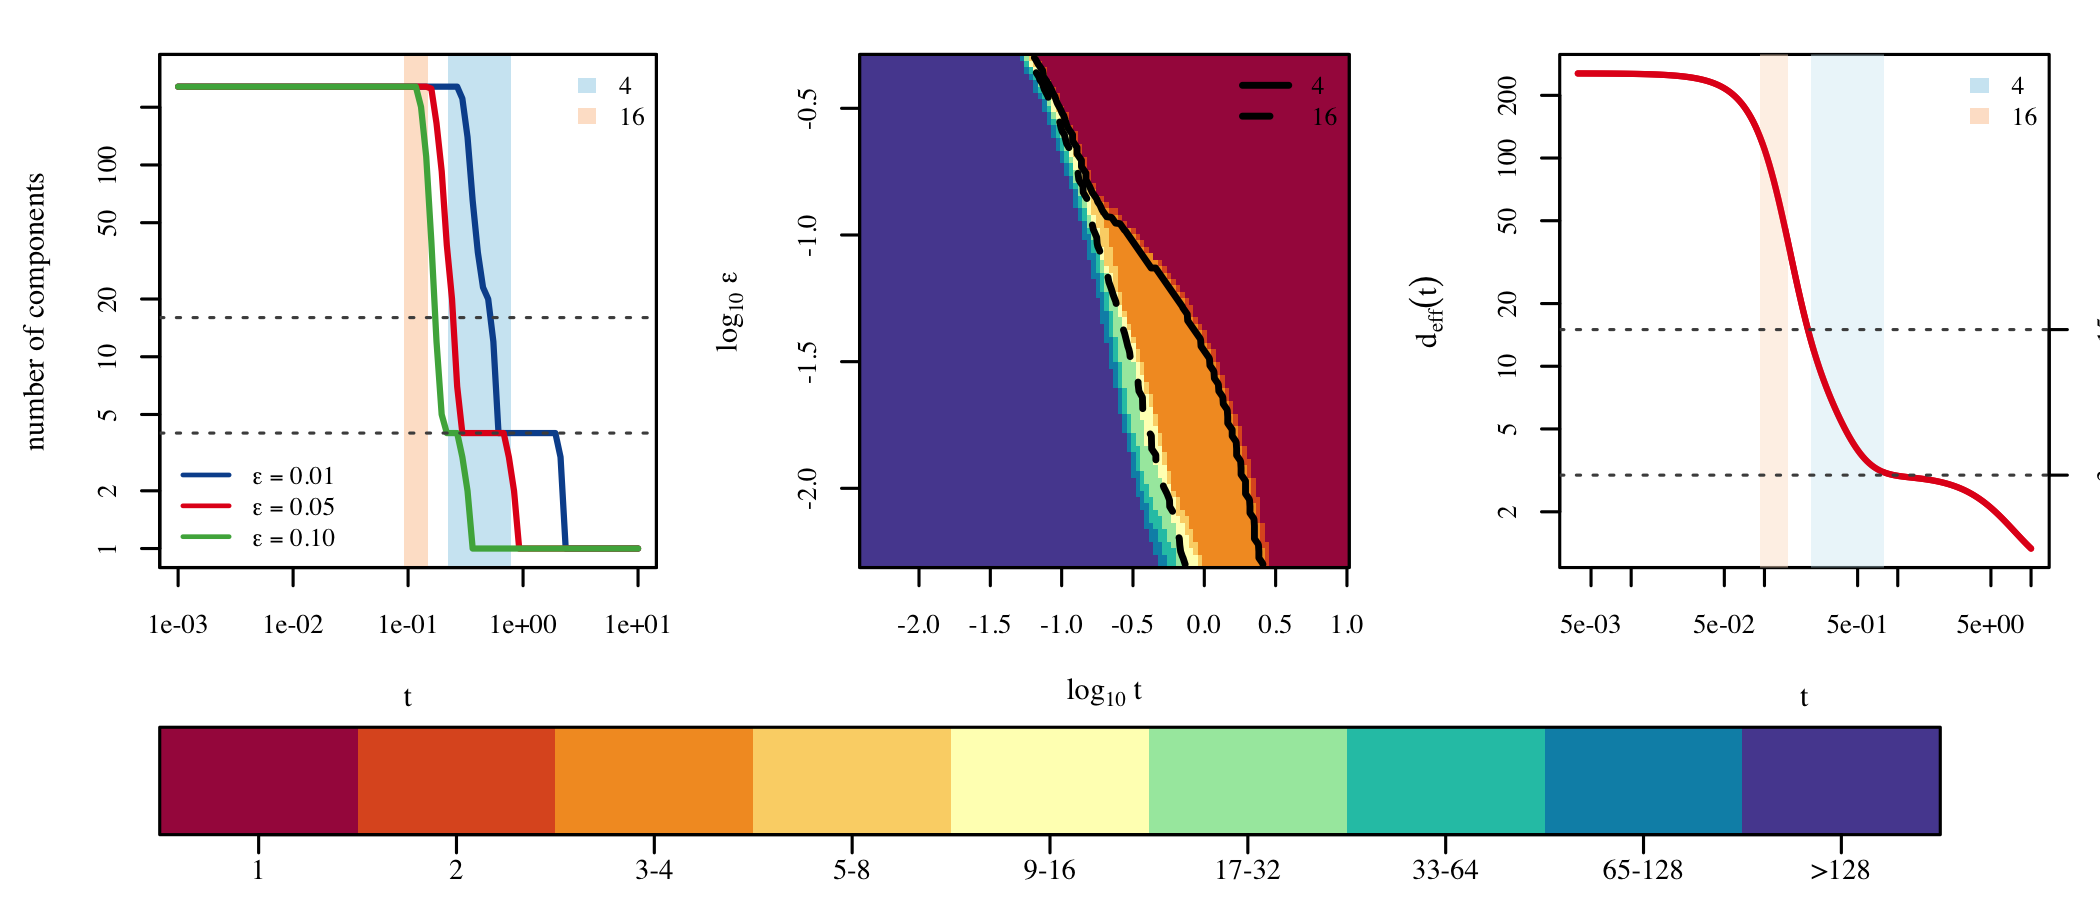
\includegraphics[width=0.98\textwidth]{F3_F4_F5_plateaus_geometry.png}
  \caption[Component plateaus and diffusion geometry]{Component count plateaus and diffusion geometry for the 13-4 network. Left: Component count $n_{\mathrm{comp}}(t)$ of the $\varepsilon$-thresholded diffusion network $\mathcal{D}_T(t)$ for distance thresholds $\varepsilon \in \{0.01, 0.05, 0.10\}$ using single-linkage clustering (SLINK), with shaded predicted spectral gap windows. Center: Contour map of $n_{\mathrm{comp}}(t, \varepsilon)$ over the logarithmic time-threshold plane ($t \in [0.004, 10]$ and $\varepsilon \in [0.005, 0.50]$); nearly vertical contour lines confirm threshold-robustness of community detection, validating the SLINK method. Right: Effective embedding dimension $d_{\mathrm{eff}}(t)$ vs dynamic time $t$, displaying step-wise drops across the predicted 16-community and 4-community plateau windows.}
  \label{fig:plateaus_geometry_combined}
\end{figure*}

Using the SLINK algorithm \cite{sibson1973}, we compute single-linkage merge heights on $d_t(i,j)$ to determine the component count $n_{\mathrm{comp}}(t)$ of $\mathcal{D}_T(t)$ across time (Figure~\ref{fig:plateaus_geometry_combined}, Left). Table~\ref{tab:plateaus} compares predicted plateau lengths in $\log_{10} t$ against empirical measurements.

\begin{table}[t]
\caption[Predicted vs measured plateau extent]{Predicted vs measured plateau extent in log-time for network 13-4.}
\label{tab:plateaus}
\begin{ruledtabular}
\begin{tabular}{lcccc}
Network & $m$ & $\lambda_{m+1}/\lambda_m$ & Predicted ($\log_{10}$) & Measured ($\log_{10}$) \\
\hline
13-4 & 4  & 3.64 & 0.545 & 0.360 \\
13-4 & 16 & 1.64 & 0.209 & 0.000 \\
\end{tabular}
\end{ruledtabular}
\end{table}

Figure~\ref{fig:plateaus_geometry_combined} (Center) displays the full $(t, \epsilon)$ plane. The vertical orientation of contour lines at $n_{\mathrm{comp}}=4$ demonstrates that community detection is robust to the choice of distance threshold $\epsilon$ (or correlation threshold $T$), depending purely on physical time $t$. In Figure~\ref{fig:plateaus_geometry_combined} (Right), the effective dimension $\deff(t)$ decreases monotonically with time, exhibiting clear steps matching the 16-community and 4-community plateau windows before converging to 1. Intuitively, this validates the theoretical result that the mapping from network phase states on the nodes to the diffusion embedding results in a point cloud shrinking to a single point, as the dynamics approach synchronization.

\paragraph{Hub Damage Mechanism.} 

\begin{figure*}[t]
  \centering
  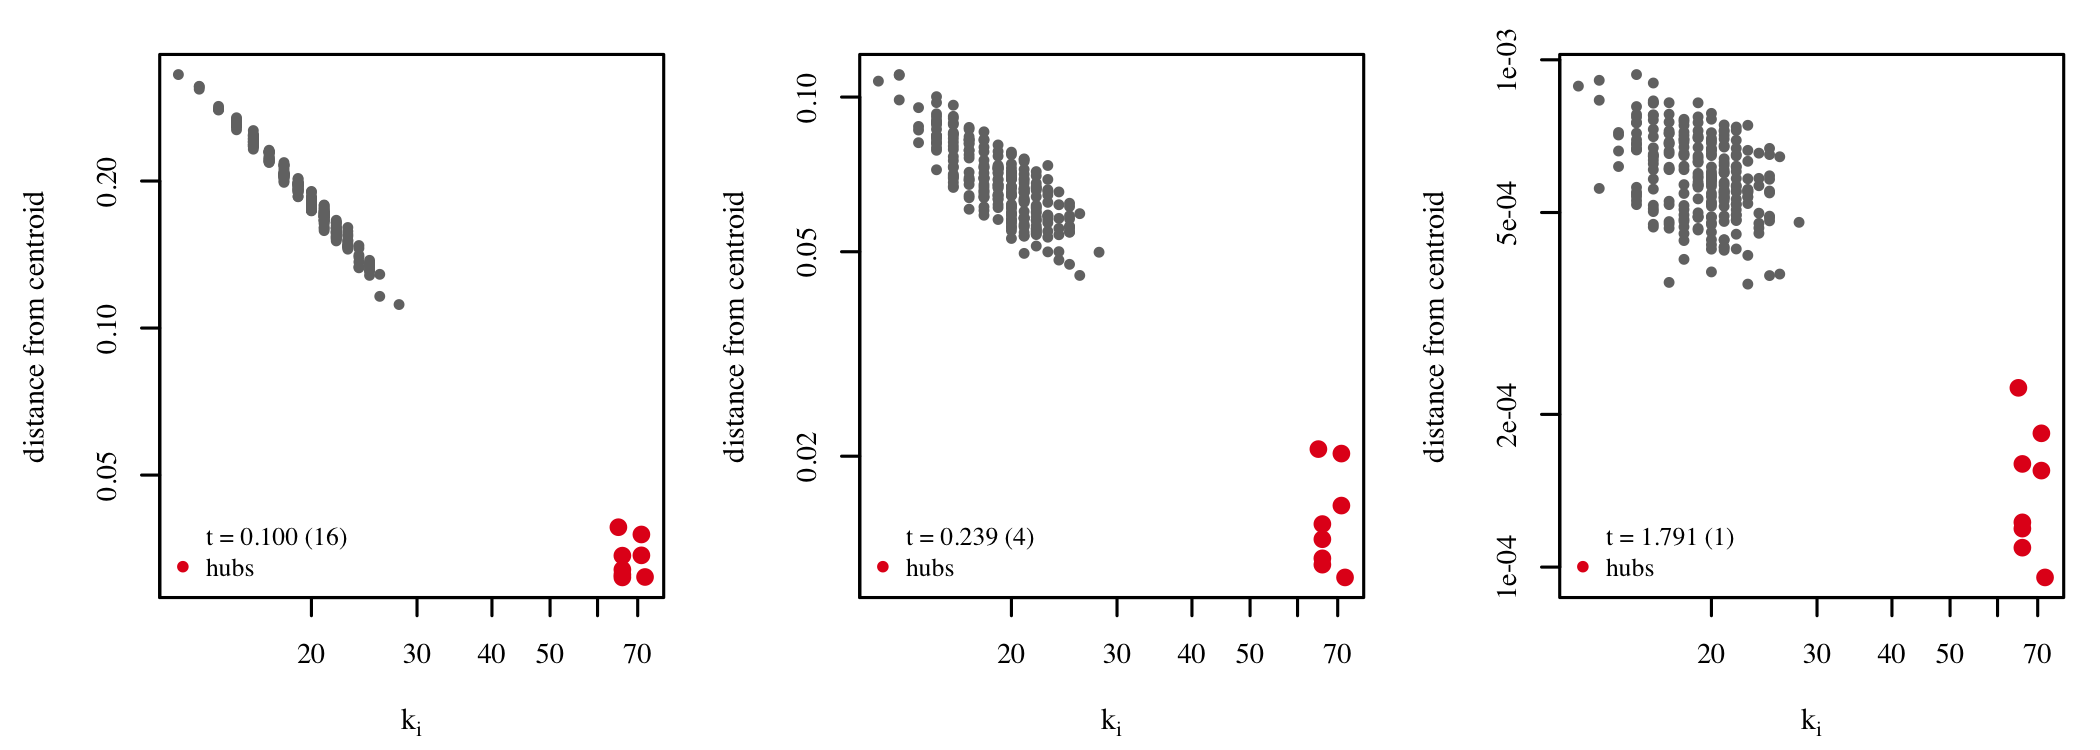
\includegraphics[width=0.98\textwidth]{F6_hubs_test.png}
  \caption[Hub distance from centroid across diffusion times]{Node distance from diffusion centroid versus degree $k_i$ after adding 8 random hubs, shown at three dynamic diffusion times ($t = 0.038$ in 16-community window, $t = 0.420$ in 4-community window, $t = 1.346$ fully merged). Hubs tend to stay close to the centroid of the diffusion embedding point cloud. As the system evolves, the rest of the nodes apporach the hubs.}
  \label{fig:hubs_test}
\end{figure*}

\begin{figure*}[t]
  \centering
  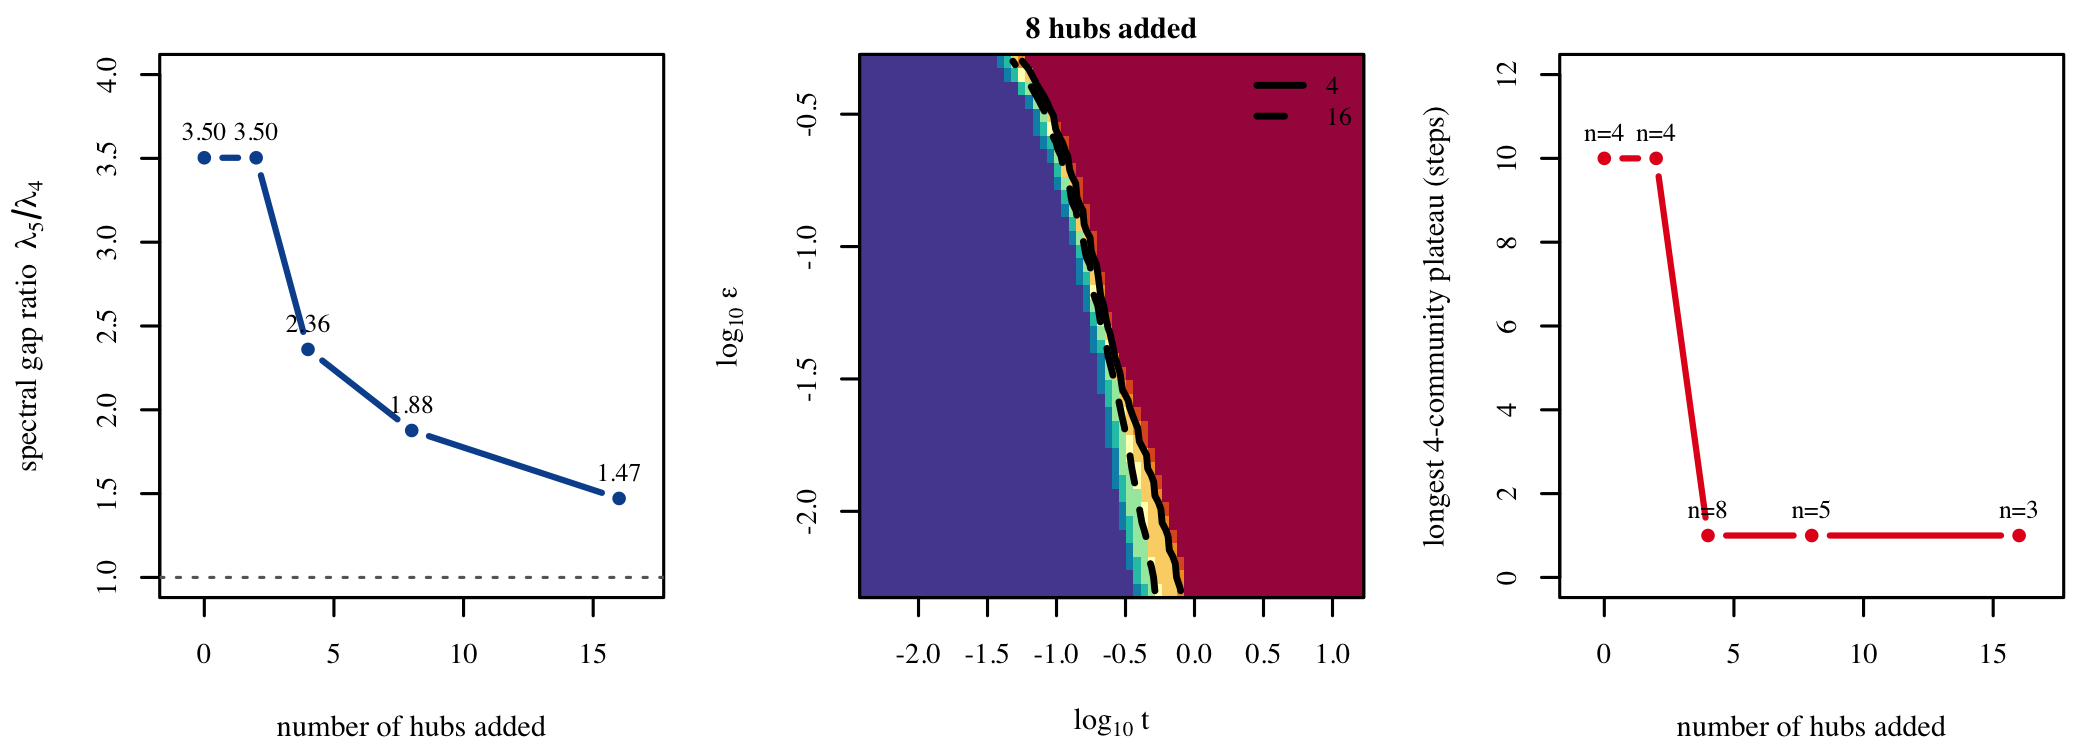
\includegraphics[width=0.98\textwidth]{F7_hub_damage.png}
  \caption[Plateau destruction by degree heterogeneity]{Plateau destruction by degree heterogeneity (hubs). Left panel: Spectral gap ratio $\lambda_5/\lambda_4$ versus number of added hubs $n_{\mathrm{hub}}$, showing a steady decrease from $3.50$ to $1.47$. Center panel: Contour map of $n_{\mathrm{comp}}(t, \varepsilon)$ over the logarithmic time-threshold plane after adding 8 hubs. Right panel: Longest 4-community plateau duration (in grid steps) versus number of added hubs $n_{\mathrm{hub}}$. Adding 8 hubs ($\approx 3\%$ of nodes) completely destroys the 4-community plateau.}
  \label{fig:hub_damage}
\end{figure*}

We test the impact of targeted degree heterogeneity by adding $n_{\mathrm{hub}} \in \{2, 4, 8, 16\}$ hubs (extra degree $\approx 50$) to the 13-4 network. As shown in Figure~\ref{fig:hub_damage} (Left), adding hubs increases overall inter-community connectivity, which narrows the spectral gap ratio $\lambda_5/\lambda_4$ from $3.50$ down to $1.88$ for 8 hubs. However, the primary mechanism destroying community detection is geometric: as illustrated in Figure~\ref{fig:hubs_test}, hubs sit near the centroid of diffusion space because they connect uniformly across all modules. Consequently, single-linkage clustering merges all modules through the central hub ``bridges'' at low distance thresholds (Figure~\ref{fig:hub_damage}, Center), completely destroying single-linkage plateau formation (Figure~\ref{fig:hub_damage}, Right) long before the spectral gap itself fully closes. The fragility of synchronization dynamics to the presence of hubs reveals the limitations to the applicability of this method to real-world networks, where hubs are ubiquitous.

%======================================================================
\paragraph{Structural Noise Sweep (Inter-Community Noise Sweep)}
%\label{sec:zout_sweep}

\begin{figure*}[t]
  \centering
  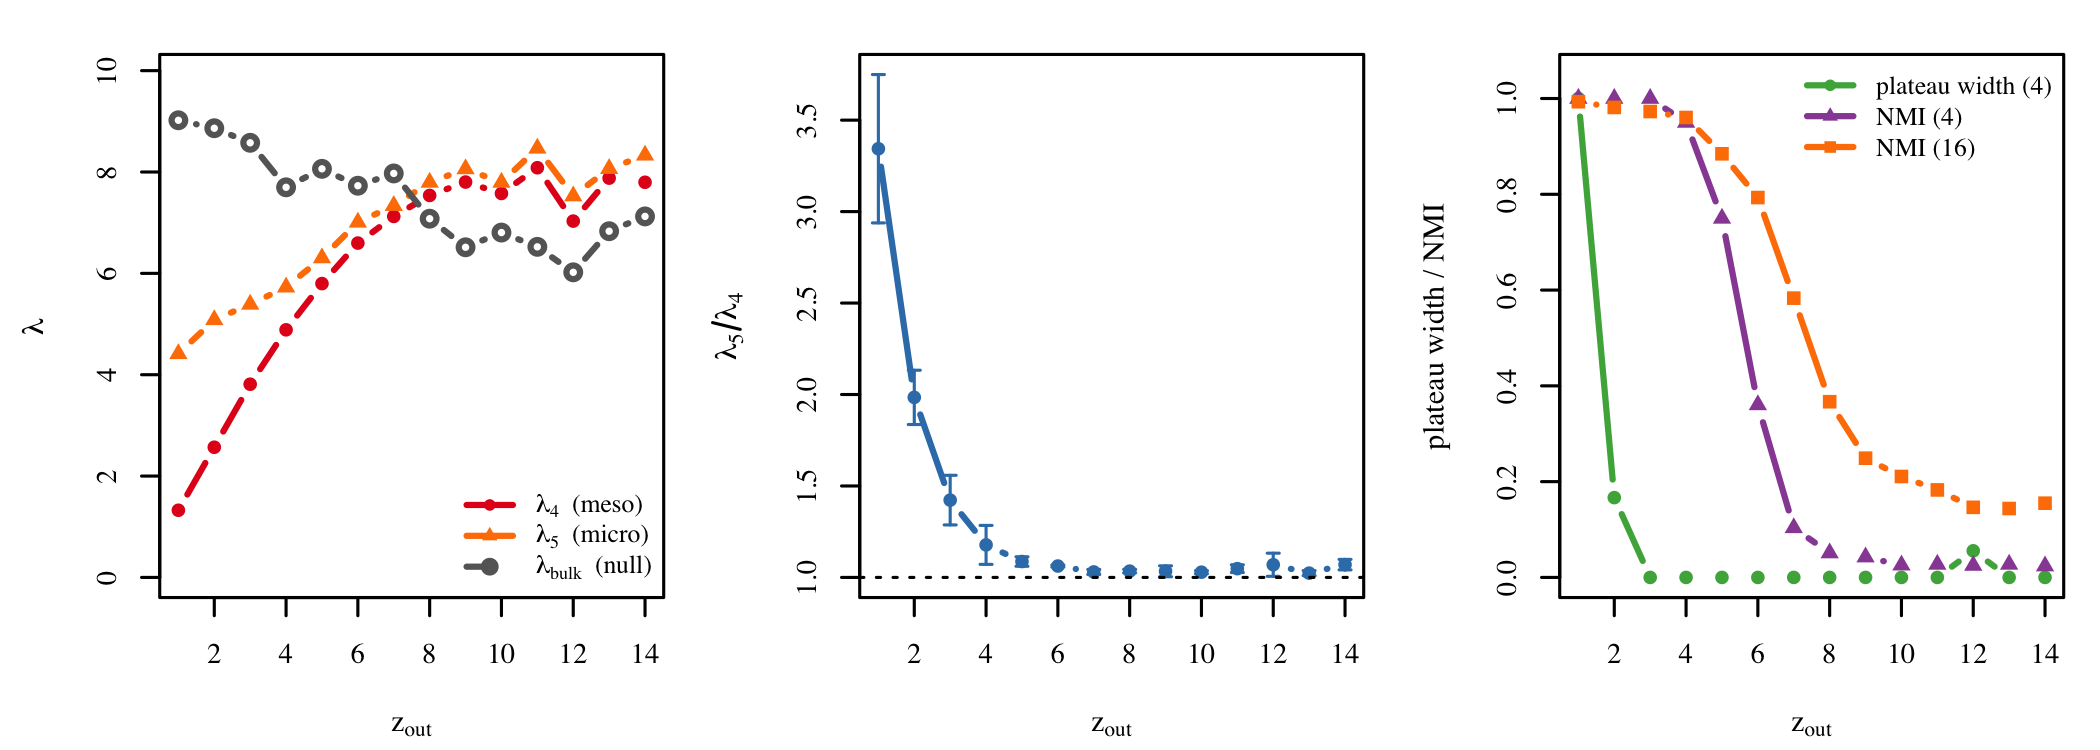
\includegraphics[width=0.98\textwidth]{F8_zout_sweep.png}
  \caption[Robustness sweep over inter-community degree]{Robustness sweep over inter-community degree $z_{\mathrm{out}} \in [1, 14]$ at fixed total degree $\langle k \rangle = 18$. Left panel plots structural eigenvalues $\lambda_4$ (meso) and $\lambda_5$ (micro) versus the bulk edge $\lambda_{\mathrm{bulk}}$ of the null model. Center panel shows the spectral gap ratio $\lambda_5/\lambda_4$. Right panel compares the normalized 4-community plateau width against Normalized Mutual Information (NMI) recovery for 4 and 16 communities.}
  \label{fig:zout_sweep}
\end{figure*}

Finally, we test robustness to structural noise by varying $z_{\mathrm{out}}$ from 1 to 14 while fixing $\langle k \rangle = 18$. We track community recovery using Normalized Mutual Information (NMI) \cite{danon2005}. Intuitively, NMI is a measure of how well the detected communities match the ground truth communities, with NMI = 1 indicating perfect recovery and NMI = 0 indicating random assignment. As shown in Figure~\ref{fig:zout_sweep}, as $z_{\mathrm{out}}$ increases:
1. The 4-community plateau width vanishes first ($z_{\mathrm{out}} \ge 2$).
2. The spectral gap ratio $\lambda_5/\lambda_4$ collapses next ($z_{\mathrm{out}} \ge 4$).
3. Community recovery measured by NMI decays last ($z_{\mathrm{out}} \ge 6$).

This is the key result: the regime in which synchronisation dynamics \textit{reveals} topological scales via plateaus is strictly narrower than the regime in which those communities remain statistically recoverable.

%======================================================================
\section{Discussion}
\label{sec:discussion}

Our results establish that synchronisation-based community detection in the linearised Kuramoto model is an exact instance of diffusion geometry. By re-formulating the pairwise order parameter $\rho_{ij}(t)$ as a diffusion kernel $\exp(-d_t^2(i,j)/2)$, we place the heuristics of Arenas \textit{et al.} on a firm mathematical footing.

The method exhibits mathematical elegance, but also two distinct failure modes: (i) sensitivity to degree heterogeneity (hubs pull coordinates to the diffusion centroid), and (ii) stringent modularity requirements for plateau formation compared to static NMI recovery. These findings provide clear scope conditions for applying diffusion geometry to empirical biological and neural networks.

\begin{acknowledgments}
This work was conducted as part of the course \emph{Physics of Complex Networks: Structure and Dynamics} (Master's Degree in Physics of Data / Physics, University of Padua).

Source code and data are available in the \href{https://github.com/filippobezzi/PoCN_projects}{repository}. 

The author acknowledges the use of generative artificial intelligence assistance (DeepMind's Antigravity AI assistant) for writing assistance, code development, data formatting, and proofreading the manuscript. All analytical derivations, mathematical proofs, numerical simulations, and physical interpretations have been rigorously verified by the author.
\end{acknowledgments}

\bibliographystyle{apsrev4-2}
\bibliography{refs}

\appendix
\phantomsection
\section{Appendix: Derivation of the Synchronisation Order Parameter‑Diffusion Embedding Distance Equivalence}\label{app:derivation}

Here we provide an explicit, step-by-step derivation of the analytical identity connecting the linearised Kuramoto order parameter $\rho_{ij}(t)$ to the graph diffusion distance $d_t(i,j)$.

\paragraph{Linearised Dynamics and Phase Covariance}
In the co-rotating frame and for small phase differences, the Kuramoto dynamics reduce to the graph heat equation:
\begin{equation}
\dot{\bm\theta}(t) = -K \Lap \bm\theta(t),
\end{equation}
whose exact solution is given by:
\begin{equation}
\bm\theta(t) = e^{-K \Lap t} \bm\theta(0).
\end{equation}
Assuming independent Gaussian initial conditions $\bm\theta(0) \sim \mathcal{N}(0, \sigma^2 \mathbb{I})$, the mean phase vector is $\langle \bm\theta(0) \rangle = \bm 0$ and the initial covariance is $\langle \bm\theta(0) \bm\theta(0)^\top \rangle = \sigma^2 \mathbb{I}$. Since $\bm\theta(t)$ is a linear transformation of $\bm\theta(0)$, $\bm\theta(t)$ remains a zero-mean Gaussian vector with covariance matrix:
\begin{equation}
\Cov(t) = \langle \bm\theta(t) \bm\theta(t)^\top \rangle = e^{-K \Lap t} \langle \bm\theta(0) \bm\theta(0)^\top \rangle e^{-K \Lap t}.
\end{equation}
Exploiting the symmetry of the graph Laplacian ($\Lap^\top = \Lap$), the matrix exponential $e^{-K \Lap t}$ is also symmetric, yielding:
\begin{equation}
\Cov(t) = \sigma^2 e^{-2K \Lap t}.
\end{equation}

\paragraph{Phase Difference Distribution and Order Parameter}
The phase difference between nodes $i$ and $j$ is $\Delta_{ij}(t) = \theta_i(t) - \theta_j(t) = (\bm e_i - \bm e_j)^\top \bm\theta(t)$. Being a linear combination of zero-mean Gaussian variables, $\Delta_{ij}(t)$ is a scalar zero-mean Gaussian variable $\Delta_{ij}(t) \sim \mathcal{N}(0, s_{ij}^2(t))$, where the variance is:
\begin{equation}
s_{ij}^2(t) = \operatorname{Var}(\theta_i - \theta_j) = C_{ii}(t) + C_{jj}(t) - 2 C_{ij}(t).
\end{equation}
The pairwise order parameter $\rho_{ij}(t) = \langle \cos(\theta_i - \theta_j) \rangle$ is the real part of the characteristic function $\phi_{\Delta_{ij}}(1) = \langle e^{i \Delta_{ij}} \rangle$. For a zero-mean Gaussian variable with variance $s_{ij}^2(t)$, the characteristic function evaluates to:
\begin{equation}
\langle e^{i \Delta_{ij}} \rangle = \exp\Big( -\frac{1}{2} s_{ij}^2(t) \Big).
\end{equation}
Since this expression is strictly real, we obtain:
\begin{equation}
\rho_{ij}(t) = \langle \cos(\theta_i - \theta_j) \rangle = \exp\Big( -\frac{1}{2} s_{ij}^2(t) \Big).
\end{equation}

\paragraph{Spectral Decomposition and Diffusion Distance}
Using the spectral expansion of the symmetric Laplacian $\Lap = \sum_{\alpha=1}^N \lambda_\alpha \bm v_\alpha \bm v_\alpha^\top$, the matrix exponential element $C_{ab}(t)$ expands as:
\begin{equation}
C_{ab}(t) = \sigma^2 \sum_{\alpha=1}^N e^{-2K \lambda_\alpha t} v_\alpha(a) v_\alpha(b).
\end{equation}
Substituting this into the variance expression $s_{ij}^2(t)$ gives:
\begin{align}
s_{ij}^2(t) &= \sigma^2 \sum_{\alpha=1}^N e^{-2K \lambda_\alpha t} \Big( v_\alpha(i)^2 + v_\alpha(j)^2 - 2 v_\alpha(i) v_\alpha(j) \Big) \nonumber \\
&= \sigma^2 \sum_{\alpha=1}^N e^{-2K \lambda_\alpha t} \big( v_\alpha(i) - v_\alpha(j) \big)^2.
\end{align}
For any connected network, the trivial ground-state eigenvector corresponding to $\lambda_1 = 0$ is uniform: $v_1(k) = 1/\sqrt{N}$ for all $k$. Thus, $v_1(i) - v_1(j) = 0$, and the $\alpha = 1$ term vanishes identically from the sum. Defining the diffusion distance $d_t(i,j)$ as:
\begin{equation}
d_t^2(i,j) = \sigma^2 \sum_{\alpha=2}^N e^{-2K\lambda_\alpha t} \big( v_\alpha(i) - v_\alpha(j) \big)^2,
\end{equation}
we confirm $s_{ij}^2(t) = d_t^2(i,j)$, completing the proof of Eq.~\eqref{eq:main_identity}:
\begin{equation}
\rho_{ij}(t) = \exp\Big( -\frac{1}{2} d_t^2(i,j) \Big).
\end{equation}


\end{document}
